\section{Results}

\cref{fig:fig3} compares training and testing accuracy of the KNN model across
three preprocessing methods: raw (\texttt{df\_clean}), averaged
(\texttt{df\_avg}), and normalized (\texttt{df\_norm}). For the raw model,
optimal \(k \approx 12\) balances training and testing accuracy. The averaged
model shows flat trends, likely due to information loss from aggregation. The
normalized model performs best, with optimal \(k \approx 4\), offering balanced
and stable accuracy.

\begin{figure}[H]
	\centering
	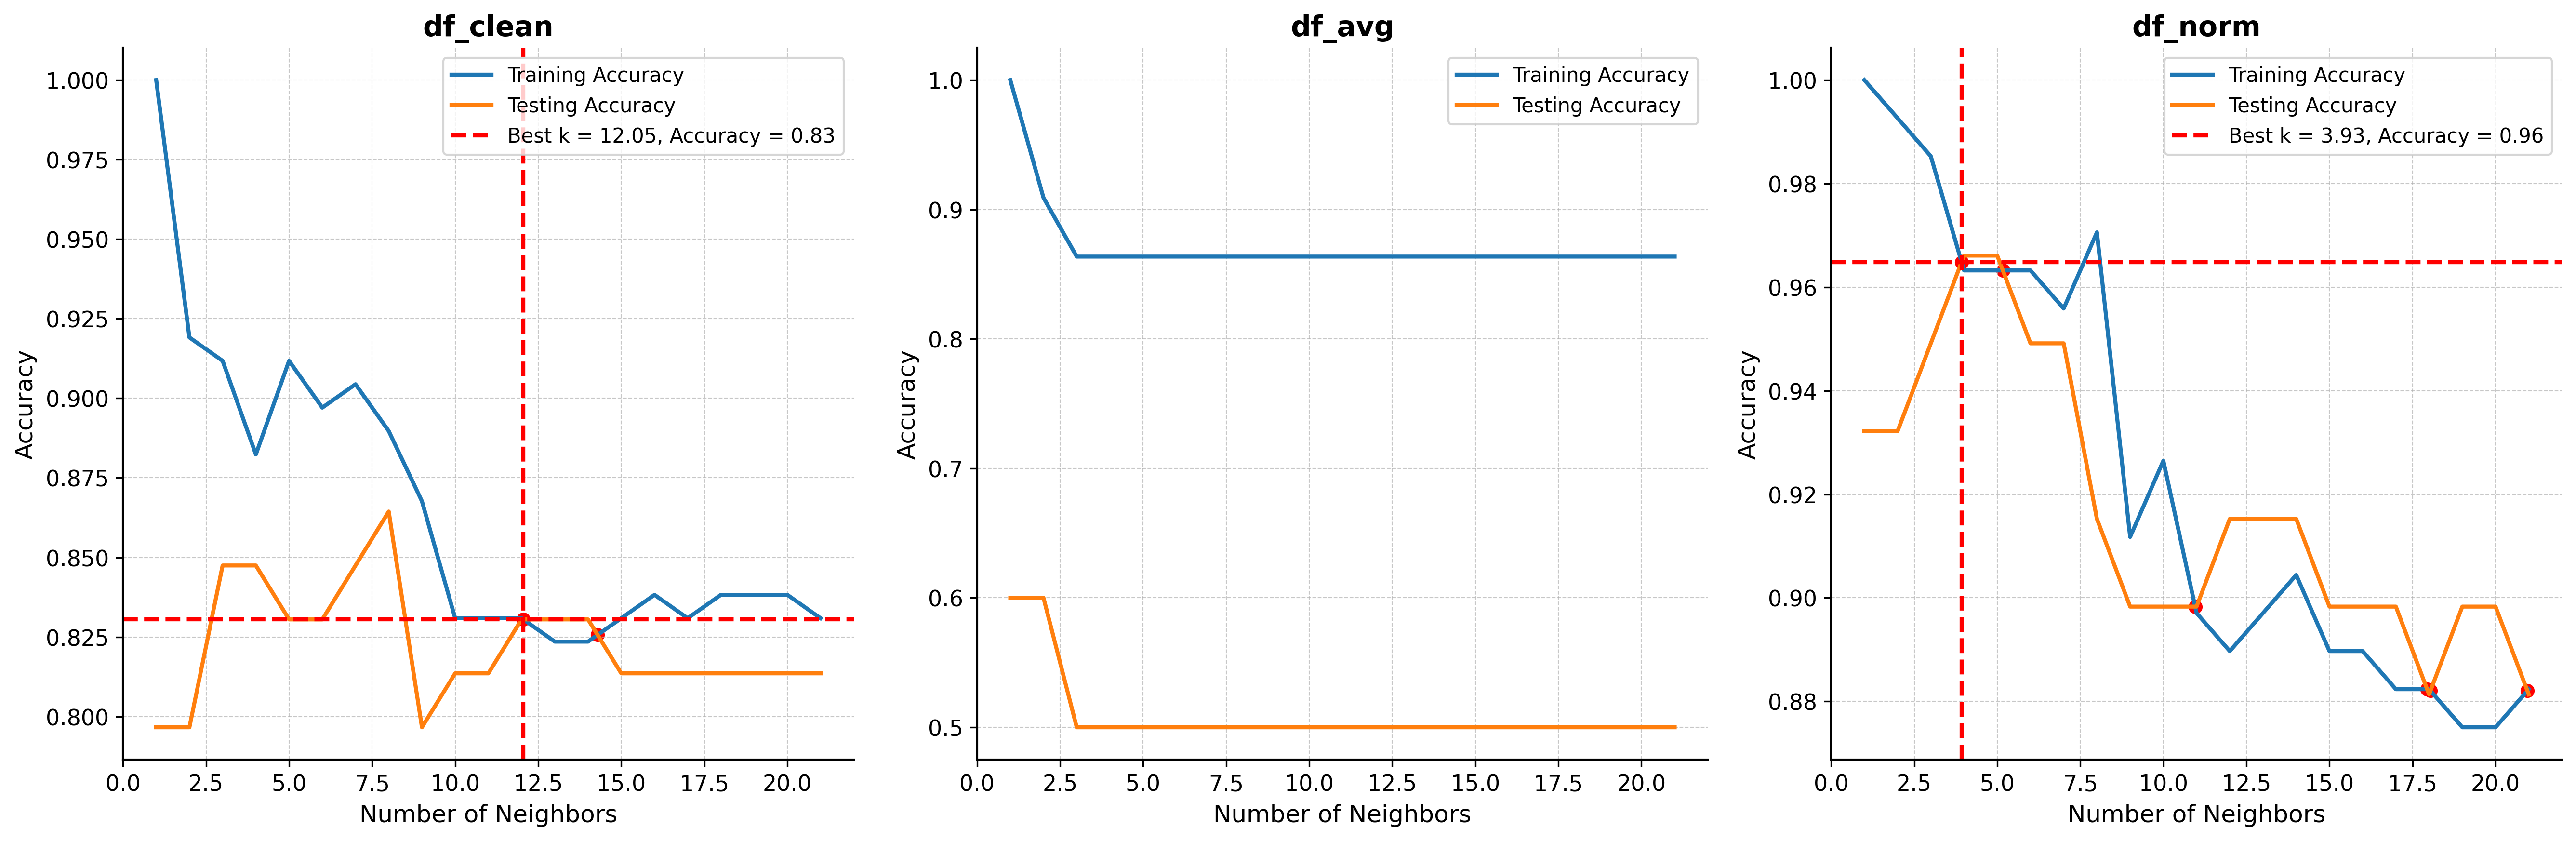
\includegraphics[width=0.99\textwidth]{../images/feature_selection/best_k.png}
	\caption{Optimal \(k\) determination using testing and training accuracy.}
	\label{fig:fig3}
\end{figure}

Finally, the last step is to integrate the whole process within an API. The
backend of this system is implemented using FastAPI. Its primary functions
include serving the frontend, managing model files, retrieving evaluation
metrics, and handling prediction requests, as shown in \cref{fig:fig4}. The
root endpoint (\texttt{/}) serves the \texttt{index.html} file, which provides
the user interface for interaction. The system organizes models into
datetime-labeled folders under \texttt{MODEL\_DIR}, where each folder
represents a distinct training session and contains model files (\texttt{.pkl})
and evaluation metrics stored in a \texttt{metrics.txt} file.

\begin{figure}[H]
	\centering
	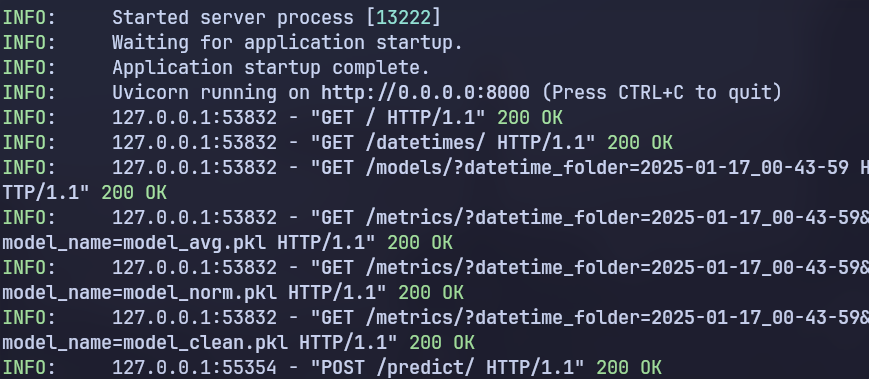
\includegraphics[width=0.75\textwidth,
		height=0.2\textheight]{../images/api/backend.png}
	\caption{Example of messages exchange between frontend and backend.}
	\label{fig:fig4}
\end{figure}

The \texttt{/datetimes/} endpoint retrieves all datetime-named folders,
enabling users to explore different model versions. Once a folder is selected,
the \texttt{/models/} endpoint lists available model files within it. The
\texttt{/metrics/} endpoint fetches and displays the content of the
\texttt{metrics.txt} file for the chosen folder, allowing users to view the
performance metrics of the associated models. The prediction process is handled
by the \texttt{/predict/} endpoint, where the user provides feature inputs and
selects a model. The backend then loads the specified model using the
\texttt{pickle} module and if the selected model is \texttt{model\_norm} it
applies min-max normalization, using pre-computed max-min values from the
normalized dataset. Predictions are generated by the model and returned as a
JSON response, indicating whether the input data corresponds to a healthy or
Parkinson's individual.

The frontend was built using HTML, CSS, and JavaScript. The \cref{fig:fig5}
shows a preview of it. Users can select datetime folders and models through
dynamically populated dropdown menus, which are updated by fetching data from
the backend endpoints \texttt{/datetimes/} and \texttt{/models/}. Additionally,
users can upload a JSON file containing feature values, and the uploaded data
automatically populates the input fields, simplifying the data entry process.
Metrics for the selected model are retrieved via the \texttt{/metrics/}
endpoint and displayed directly on the page to provide insights into the
model's performance.

\begin{figure}[H]
	\centering
	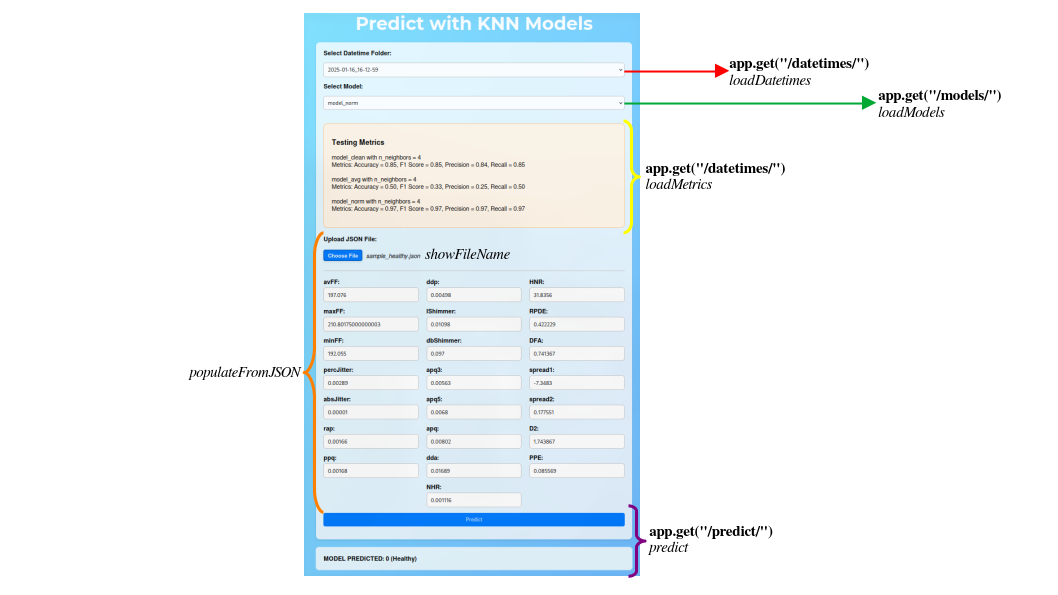
\includegraphics[width=0.95\textwidth,height=0.30\textheight]{../images/api/frontend.png}
	\caption{Frontend preview with annotated elements: functions related to the
		backend are shown in \textbf{bold}, while functions specific to the frontend
		are highlighted in \textit{italics}.}
	\label{fig:fig5}
\end{figure}

The frontend handles form submissions by sending a POST request to the
\texttt{/predict/} endpoint with the user-provided inputs and the selected
model. The backend processes the request, and the prediction results are
displayed directly on the webpage. JavaScript functions manage dynamic
interactions, such as loading datetime folders, model files, and metrics, as
well as validating uploaded JSON files and showing prediction outputs.
